%!TEX root = draft.tex
\section{Definitions and Proofs of Section \ref{sec:simulation and refinement}}
\label{sec:appendix definitions and proofs of section simulation and refinement}


{\noindent \bf Theorem \ref{theorem:equivalence of our simulation and refinement}}: Given LTS $A$ and deterministic $B$, and functions $f_s,f_t$, such that $P_{(f_s,f_t)}$ holds. Then, B $f_t$-refines $A$, if and only if there exists a $f_s$-simulation relation between $A$ and $B$.

\begin {proof}
Assume $A = (Q_A,\Sigma_A,\rightarrow_a,q_{0A})$ and $B = (Q_B,\Sigma_B,\rightarrow_b,q_{0B})$.

For the $\textit{if}$ direction. Assume $R$ is a $f_s$-simulation relation between $A$ and $B$. Given $q_{1A},\ldots,q_{kA} \in Q_A$, $q_{1B},\ldots,q_{kB}$, $\alpha_1,\ldots,\alpha_k$, such that

\begin{itemize}
\setlength{\itemsep}{0.5pt}
\item[-] $\forall 0 \leq i < k$, $q_{iA} {\xrightarrow{\alpha_{i+1}}}_a q_{i+1A}$,

\item[-] $\forall 0 \leq i \leq k$, $(q_{iA},q_{iB}) \in R$, and

\item[-] $\forall 0 \leq i < k$, $q_{iB} {\xrightarrow{f_s(q_{iA},q_{iB},\alpha_{i+1})}}_b q_{i+1B}$.
\end{itemize}

We can see that, given execution $t_A = \alpha_1 \cdot \ldots \cdot \alpha_k$ of $A$, by $f_s$-simulation, we have execution $t_b = f_s(q_{0A},q_{0B},\alpha_1) \cdot \ldots \cdot f_s(q_{k-1A},q_{k-1B},\alpha_k)$ of $B$.

Since $P_{(f_s,f_t)}$ holds, we can see that

\begin{itemize}
\setlength{\itemsep}{0.5pt}
\item[-] $f_t(\alpha_1) = f_s(q_{0A},q_{0B},\alpha_1)$.

\item[-] $f_t(\alpha_1 \cdot \alpha_2) = f_s(q_{1A},q'_{1B},\alpha_2)$. Here $q'_{1B}$ is obtained from $q_{B0}$ by doing $\alpha_1$ transitions. Since $B$ is deterministic, it is easy to see that $q'_{1B} = q_{1B}$, and $f_t(\alpha_1 \cdot \alpha_2) = f_s(q_{1A},q_{1B},\alpha_2)$.

$\ldots$

\item[-] $f_t(\alpha_1 \cdot \ldots \cdot \alpha_k) = f_s(q_{k-1A},q'_{k-1B},\alpha_k)$. Here $q'_{k-1B}$ is obtained from $q_{B0}$ by doing $\alpha_1 \cdot \ldots \cdot \alpha_{k-1}$ transitions. Since $B$ is deterministic, it is easy to see that $q'_{k-1B} = q_{k-1B}$, and $f_t(\alpha_1 \cdot \ldots \cdot \alpha_k) = f_s(q_{k-1A},q_{k-1B},\alpha_k)$.
\end{itemize}

We can see that $t_B = f_t(\alpha_1) \cdot \ldots \cdot f_t(\alpha_1 \cdot \ldots \cdot \alpha_k)$. Therefore, by definition of $f_t$-refinement, we can see that B $f_t$-refines $A$.


For the $\textit{only if}$ direction. Assume $B$ $f_t$-refines $A$. Let a relation $R_t$ be defined as follows: Given $q_A \in Q_A$ and $q_B \in Q_B$, $(q_A,q_B) \in R_t$, if $\exists \alpha_1, \ldots, \alpha_k \in \Sigma_A$, $\exists q_{1A},\ldots,q_{k-1A} \in Q_A$, and $\exists q_{1B},\ldots,q_{k-1B} \in Q_B$, such that $q_{0A} {\xrightarrow{\alpha_1}}_a q_{1A} \ldots {\xrightarrow{\alpha_{k-1}}}_a q_{k-1A} {\xrightarrow{\alpha_k}}_a q_A$, and $q_{0B} {\xrightarrow{f_t(\alpha_1)}}_b q_{1B} \ldots$ ${\xrightarrow{f_t(\alpha_1 \cdot \cdot \ldots \cdot \alpha_{k-1})}}_b q_{k-1B} {\xrightarrow{f_t(\alpha_1 \cdot \ldots \cdot \alpha_k)}}_b q_B$.

Let us now prove that $R_t$ is a $f_s$-simulation relation. Assume that $q_A {\xrightarrow{\alpha}}_a q'_A$. Then we can see that $q_{0A} {\xrightarrow{\alpha_1}}_a q_{1A} \ldots {\xrightarrow{\alpha_{k-1}}}_a q_{k-1A} {\xrightarrow{\alpha_k}}_a q_A {\xrightarrow{\alpha}}_A q'_A$ and $\alpha_1 \cdot \ldots \cdot \alpha_k \cdot \alpha$ is an execution of $A$.

By assumption, $B$ $f_t$-refines $A$. Therefore, $f_t(\alpha_1) \cdot \ldots \cdot f_t(\alpha_1 \cdot \ldots \cdot \alpha_k) \cdot f_t(\alpha_1 \cdot \ldots \cdot \alpha_k \cdot \alpha)$ is an execution of $B$. Since $B$ is deterministic, we can see that $\exists q'_B$, such that $q_{0B} {\xrightarrow{f_t(\alpha_1)}}_b q_{1B} \ldots$ ${\xrightarrow{f_t(\alpha_1 \cdot \cdot \ldots \cdot \alpha_{k-1})}}_b q_{k-1B} {\xrightarrow{f_t(\alpha_1 \cdot \ldots \cdot \alpha_k)}}_b q_B {\xrightarrow{f_t(\alpha_1 \cdot \ldots \cdot \alpha_k \cdot \alpha)}}_b q'_B$. By definition, we can see that $(q'_A,q'_B) \in R_t$.

Since $P_{(f_s,f_t)}$ holds, we have that $f_t(\alpha_1 \cdot \ldots \cdot \alpha_k \cdot \alpha) = f_s(q_A,q''_B,\alpha)$, where $q''_B$ is obtained from $q_{0B}$ by doing $f_t(\alpha_1) \cdot \ldots \cdot f_t(\alpha_1 \cdot \ldots \cdot \alpha_k)$ transitions. Since $B$ is deterministic, we can see that $q''_B = q_B$ and $f_t(\alpha_1 \cdot \ldots \cdot \alpha_k \cdot \alpha) = f_s(q_A,q_B,\alpha)$. We can see that $q_B {\xrightarrow{f_s(q_A,q_B,\alpha)}}_b q'_B$. Therefore, $R_t$ is a $f_s$-simulation relation. \qed
\end {proof}

\forget
{
The $\textit{only if}$ direction is obvious.

Let us prove the $\textit{if}$ direction. By assumption we already have that $RImp(Spec)$ trace refines $\llbracket imp \rrbracket$. Assume $\llbracket imp \rrbracket = (Q_{imp},\Sigma_{imp},\rightarrow_{imp},q_{0imp})$ and $RImp(Spec) = (Q_s,\Sigma_s,vis,q_{0s},li,\rightarrow_s,livReq)$. A relation $R \subseteq Q_{imp} \times Q_s$ is defined as follows: $(q_i,q_s) \in R$, if $\exists t_{imp} = \alpha_1 \cdot \ldots \cdot \alpha_k,t_s = \beta_1 \cdot \ldots \cdot \beta_k, q_{1imp}, \ldots, q_{kimp}, q_{1s}, \ldots, q_{ks}$, such that $q_{0imp} {\xrightarrow{\alpha_1}}_{imp} q_{1imp} \ldots {\xrightarrow{\alpha_k}}_{imp} q_{kimp}$ is an execution of $\llbracket imp \rrbracket$, $q_{kimp}=q_i$, $q_{0s} {\xrightarrow{\beta_1}}_s q_{1s} \ldots {\xrightarrow{\beta_k}}_s q_{ks}$ is an execution of $RImp(Spec)$, $q_{ks}=q_s$, and $t_{imp}$ and $t_s$ correspond. Let us prove that $R$ is a simulation relation. Note that, given $t_{imp}$, there exists at most one $t_s$, such that $t_{imp}$ and $t_s$ correspond.

\begin{itemize}
\setlength{\itemsep}{0.5pt}
\item[-] If $q_{imp} {\xrightarrow{m(a,b,r)}}_{imp} q'_{imp}$: It is easy to see that $t'_{imp} = t_{imp} \cdot m(a,b,r) \in \llbracket imp \rrbracket$.

Since $RImp(Spec)$ trace refines $\llbracket imp \rrbracket$, there exists $t'_s$ of $RImp(Spec)$, such that $t'_{imp}$ and $t'_s$ correspond.

Since given a trace $t$ of $\llbracket imp \rrbracket$, there exists at most one trace $t'$ of $RImp(Spec)$, such that $t$ and $t'$ correspond. It is easy to see that such $t'_s$ is unique.

Since $t_{imp}$ and $t_s$ correspond and $RImp(Spec)$ is deterministic, we can see that $t'_s = t' \cdot m(a,b,r)$ is an execution of $RImp(Spec)$. Let $q_{ks} {\xrightarrow{m(a,b,r)}}_s q'_s$ It is easy to see that $t'_{imp}$ and $t'_s$ correspond. Therefore, $(q'_{imp},q'_s) \in R$.

\item[-] If $q_{imp} {\xrightarrow{apply(m)}}_{imp} q'_{imp}$: It is easy to see that $t'_{imp} = t_{imp} \cdot apply(m) \in \llbracket imp \rrbracket$.

Since $RImp(Spec)$ trace refines $\llbracket imp \rrbracket$, there exists $t'_s$ of $RImp(Spec)$, such that $t'_{imp}$ and $t'_s$ correspond.

Since given a trace $t$ of $\llbracket imp \rrbracket$, there exists at most one trace $t'$ of $RImp(Spec)$, such that $t$ and $t'$ correspond. It is easy to see that such $t'_s$ is unique.

We already know that $t_{imp}$ and $t_s$ correspond and $RImp(Spec)$ is deterministic. It is not hard to prove that, in $q_{kimp}$ and $q_{ks}$, $\forall r_1,r_2 \in RId$, the number of messages of $q_{kimp}$ which ``use source replica $r_1$ and destination replica $r_2$ and are still not applied'' is same as the number of operation of $q_{ks}$ which ``happens on replica $r_1$ and not visible to replica $r_2$''. Therefore, there exists transition $q_{ks} {\xrightarrow{addDel(o,r)}}_s q'_s$. Here $o$ and $r$ are obtained as follows: Assume after doing $t_{imp}$, $m=(\_,r',r)$ is the $i-th$ among ``messages with source replica $r'$, destination replica $r$ and still not applied'' w.r.t the occurring order of $t_{imp}$. Then, after doing $t_s$, $o$ is the $i-th$ among ``operations which happens on replica $r'$ and not visible to replica $r$'' w.r.t the occurring order of $t_s$. Let $t'_s = t' \cdot addDel(o,r)$.

Let us prove that such $m$, $o$ and $r$ satisfies the requirements in definition of simulation relation. Since we already know that $q_{0imp} {\xrightarrow{t_{imp}}}_{imp}^* q_{kimp}$ and $q_{0s} {\xrightarrow{t_s}}_s^* q_{ks}$, it is not hard to prove that, the $i-th$ message among ``messages with source replica $r'$, destination replica $r$ and still not applied'' w.r.t the occurring order of $t_{imp}$ is the same as the $i-th$ among messages of $q_{kimp}$ with source replica $r'$ and destination replica $r$ w.r.t $<_{sd}$. Similarly, we can prove that, the $i-th$ operations among ``operations which happens on replica $r'$ and not visible to replica $r$'' w.r.t the occurring order of $t_s$ is the same as the $i-th$ among operations of $q_{ks}$ which happens on replica $r'$ and not visible to replica $r$ w.r.t $ro$. Therefore, $o$ and $r$ satisfies the requirements in definition of simulation relation.

Let us prove that $(q'_{imp},q'_s) \in R$. From above discussion, it is not hard to see that $t'_{imp}$ and $t'_s$ correspond. Therefore, $(q'_{imp},q'_s) \in R$.
\end{itemize}
}





















\section{Definitions and Proofs of Section \ref{sec:reference implementation}}
\label{sec:appendix definitions and proofs of section reference implementation}


The following lemma states the relation between annotated history of a trace of $RImp(Spec)$ and the state of $RImp(Spec)$ at the end of this trace. 

\begin{lemma}
\label{lemma:relation between the state of RImpSpec and the annotated history}
$q_0 {\xrightarrow{\alpha_1}} q_1 \ldots {\xrightarrow{\alpha_k}} q_k$ of $RImp(Spec)$, let its annotated history to be $(O_k,\mathit{ro}_k,\mathit{vis}_k,\mathit{arb}_k)$ and $q_k = (O'_k,\mathit{ro}'_k,\mathit{del}'_k,\mathit{arb}'_k)$. Then, 
\begin{itemize}
\setlength{\itemsep}{0.5pt}
\item[-] $O'_k$ is the set of update operations of $O_k$.

\item[-] $\mathit{ro}'_k = \mathit{ro}_k \uparrow_{( O \times O )}$,

\item[-] $( \mathit{del}'_k \cdot \mathit{ro} ) \uparrow_{(O \times O)} = \mathit{vis}_k$,

\item[-] $\mathit{arb}'_k = \mathit{arb}_k$.
\end{itemize}
\end{lemma}
\begin {proof} 

We prove this lemma by induction on $k$. When $k=1$, this holds trivially. 

Assume that this holds for some $u$, and let us consider the case of $u+1$:  

\begin{itemize}
\setlength{\itemsep}{0.5pt}
\item[-] If $\alpha_{u+1} = addDel(o,r)$: $(O'_u,\mathit{ro}'_u,\mathit{del}'_u,\mathit{arb}'_u) {\xrightarrow{addDel(o,r)}} (O'_u,\mathit{ro}'_u,\mathit{del}'_u \cup \{ (o,r) \},\mathit{arb}'_u)$. This still holds. 

\item[-] If $m$ is a query method and $\alpha_{u+1} = m(a,b,r,\mathit{arb}'_u)$: $(O'_u,\mathit{ro}'_u,\mathit{del}'_u,\mathit{arb}'_u) {\xrightarrow{(m,a,b,r,\mathit{arb}'_u)}} (O'_u,\mathit{ro}'_u,\mathit{del}'_u,\mathit{arb}'_u)$. This still holds. 
\end{itemize}

This completes the proof of this lemma. $\qed$
\end {proof}







{\noindent \bf Theorem \ref{lemma:executions of reference implementation are SRV consistent}}: $\forall t \in \llbracket RImp(Spec) \rrbracket$, $anHis(t)$ is SRVC consistent w.r.t $Spec$. 

\begin {proof}

Assume $RImp(Spec) = (Q,\Sigma,q_0,\rightarrow)$, $t = \alpha_1, \ldots, $ and $q_1,\ldots \in Q$, such that $q_0 {\xrightarrow{\alpha_1}} q_1 \ldots$. Let $anHis(t) = (O_1,\mathit{ro}_1,\mathit{vis}_1,\mathit{arb}_1)$. 

According to the construction of $absT(t)$, it is easy to see that $\mathit{ro}_1 \subseteq \mathit{vis}_1$ and $\mathit{vis}_1$ is acyclic. Then, $\textit{THINAIR}$ holds.

\noindent {\bf Relation between $Q$ and annotated history}:Let $t[1,k] = \alpha_1 \cdot \ldots \cdot \alpha_k$. Given the annotated history $anHis(t[1,k]) = (O_k,\mathit{ro}_k,\mathit{vis}_k,\mathit{arb}_k)$ of $t[1,k]$, assume that $q_k = (O,\mathit{ro},\mathit{del},\mathit{arb})$, then, we need to prove that,

\begin{itemize}
\setlength{\itemsep}{0.5pt}
\item[-] $O$ is the set of update operations of $O_k$. 

\item[-] $\mathit{ro}= \mathit{ro}_k \uparrow_{( O \times O )}$, 

\item[-] $( \mathit{del} \cdot \mathit{ro} ) \uparrow_{(O \times O)} = \mathit{vis}_k$, 

\item[-] $\mathit{arb} = \mathit{arb}_k$. 
\end{itemize}



Given $i$, let $t[1,i] = \alpha_1 \cdot \ldots \cdot \alpha_i$. We define $absT(t[1,i]) = (O_\textit{t1i},<_{\textit{ro-t1i}},<_{\textit{vis-t1i}},<_{\textit{arb-t1i}})$ as follows:

\begin{itemize}
\setlength{\itemsep}{0.5pt}
\item[-] $O_\textit{t1i}$ is the set of operations generated during $t[1,i]$.

\item[-] $<_{\textit{ro-t1i}} = <_{r_1} \cup \ldots \cup <_{r_{\vert \mathbb{R} \vert}}$, where for each $i$, $<_i$ is the occurring order of operations with the $i$-th identifier in $\mathbb{R}$ over $t[1,i]$.

\item[-] $(o_1,o_2) \in <_{\textit{vis-t1i}}$, if one of the following case holds: (1) $o_1$ is delivered into replica of $o_2$, and then $o_2$ happens, (2) $o_1$ and $o_2$ are of same replica and $o_1$ happens earlier than $o_2$.

\item[-] $<_{\textit{arb-t1i}}$ is the union of arbitration order of $q_1,\ldots,q_i$.
\end{itemize}


When $m$ is a query method and assume that $absT(t)[j]=(m(a,b),rid,oid)=o$. By construction of $RImp(Spec)$, we can see that (1) $(O,ro,del,arb,vis) {\xrightarrow{m(a,b,r,arb)}} (O,ro,del,arb,vis)$, (2) $q_{\textit{i-1}} = q_i = (O,ro,del,arb,vis)$, and (3) $\textit{li-s}((O,ro,del,arb,vis),r,o) = (O',<',arb \uparrow_{O'}) \in Spec(m(a,b))$ and $o \notin O$ for some $O'$.

Assume $absT(t[1,j]) = (O_\textit{t1j},<_{\textit{ro-t1j}},<_{\textit{vis-t1j}},<_{\textit{arb-t1j}})$. It is easy to see that (1) $O$ is the set of update operations of $O_\textit{t1j}$, (2) $<_{\textit{ro-t1j}} \uparrow_{O} = ro$, (3) $<_{\textit{vis-t1j}} \uparrow_{O} = vis$, and $<_{\textit{arb-t1j}} = arb$. It is easy to see that $\textit{li-s}((O,ro,del,arb,vis),r,o)$ can be used as local interpretation of $o$.


When $m$ is an update method and assume that $absT(t)[j]=(m(a,b),rid,oid)=o$. By construction of $RImp(Spec)$, we can see that (1) $q_{\textit{i-1}} = (O,ro,del,arb,vis) {\xrightarrow{m(a,b,r,arb')}} q_i = (O \cup \{ o \},ro \oplus o ,del \oplus o,arb',(del \oplus o) \cdot (ro \oplus o))$, (2) $li((O,ro,del,arb,vis),r,o) = (O',\_,arb' \uparrow_{(O' \cup \{ o \})}) \in Spec(m(a,b))$ for some $O'$ and $o \notin O$.

Assume $absT(t[1,j]) = (O_\textit{t1j},<_{\textit{ro-t1j}},<_{\textit{vis-t1j}},<_{\textit{arb-t1j}})$. It is easy to see that (1) $O$ is the set of update operations of $O_\textit{t1j}$, (2) $<_{\textit{ro-t1j}} \uparrow_{O} = ro \oplus o$, (3) $<_{\textit{vis-t1j}} \uparrow_{O} = (del \oplus o) \cdot (ro \oplus o)$, and $<_{\textit{arb-t1j}} = arb'$. It is easy to see that $\textit{li-s}((O,ro,del,arb,vis),r,o)$ can be used as local interpretation of $o$.

Therefore, $\textit{RVAL}$ holds.

Note that, since in every step of transitions of $RImp(Spec)$ from $(O,ro,del,arb,vis)$ to $(O',ro',del',arb',vis')$, if $(o_1,o_2) \in arb$, then $(o_2,o_1) \notin arb'$. This is the reason of $<_{\textit{arb-t1j}} = arb$. $\qed$
\end {proof}






{\noindent \bf Lemma \ref{lemma:RImpcdSpec contains all the sequences of RImpSpec that are causal delivery}}: $\llbracket RImp(Spec)_{\textit{cd}} \rrbracket = \{ t \vert t \in \llbracket RImp(Spec) \rrbracket \wedge t$ satisfies causal delivery $\}$.

\begin {proof}

Let us prove the $\subseteq$ direction. We prove it by contradiction. Assume $\exists t =\alpha_1 \cdot \ldots \cdot \alpha_k \in \llbracket RImp(Spec)_{\textit{cd}} \rrbracket$ and $t$ does not satisfy causal delivery. Then there exists operations $o_1,o_2$ and replica $r$, such that $o_1 <_{hb} o_2$ and in $t$, when $o_2$ is delivered to replica $r$, $o_1$ has not been delivered to replica $r$ yet.

Let $q_1,\ldots,q_k$ be the states, such that $q_0 {\xrightarrow{\alpha_1}} q_1 \ldots {\xrightarrow{\alpha_k}} q_k$. It is easy to prove by induction that, for each $i$, when both $o_1$ and $o_2$ are in $q_i$, $(o_1,o_2)$ is in the $(ro \cup del)^*$ of $q_i$. Let $\alpha_j$ be the delivery of $o_2$ to replica $r$. In $q_{\textit{j-1}} = (O_{\textit{j-1}},ro_{\textit{j-1}},del_{\textit{j-1}},arb_{\textit{j-1}},vis_{\textit{j-1}})$, we can see that $(o_1,o_2) \in (ro_{\textit{j-1}} \cup del_{\textit{j-1}})^*$ and both $o_1,o_2 \in \{ o' \vert (o',r) \notin vis_{\textit{j-1}}, \forall o'' \in O_{\textit{j-1}}$  with replica $r, (o',o'') \notin vis_{\textit{j-1}} \}$. Then we can not do $addDel(o_2,r)$ transition, contradiction happens.

Let us prove the $\supseteq$ direction. We prove its contrapositive. Assume that $t_1 =\alpha_1 \cdot \ldots \cdot \alpha_k \notin \llbracket RImp(Spec)_{\textit{cd}} \rrbracket$, we need to prove that $t_1 \notin \{ t \vert t \in \llbracket RImp(Spec) \rrbracket \wedge t$ satisfies causal delivery $\}$. This holds trivially when $t_1 \notin \llbracket RImp(Spec) \rrbracket$.

Let us consider the case when $t \in \llbracket RImp(Spec) \rrbracket$ and $t_1 \notin \llbracket RImp(Spec)_{\textit{cd}} \rrbracket$. Let $\alpha_j$ be the first label of $t$ that makes $t$ not in $\llbracket RImp(Spec)_{\textit{cd}} \rrbracket$. Such $\alpha_j$ must be $addDel$ transition that violates the requirements of $RImp(Spec)_{\textit{cd}}$. Assume that $q_{\textit{j-1}} = (O_{\textit{j-1}},ro_{\textit{j-1}},del_{\textit{j-1}},arb_{\textit{j-1}},vis_{\textit{j-1}})$. There must exists $o_3,o_4 \in O_{\textit{j-1}}$, such that $(o_3,o_4) \in (ro_{\textit{j-1}} \cup del_{\textit{j-1}})^*$, $o_3,o_4 \in \{ o' \vert (o',r) \notin vis_{\textit{j-1}}, \forall o'' \in O_{\textit{j-1}}$  with replica $r, (o',o'') \notin vis_{\textit{j-1}} \}$, and $\alpha_j$ adds delivery of $o_2$. This violates the causal delivery. $\qed$
\end {proof}




{\noindent \bf Lemma \ref{lemma:Minus for OR-set is correct}}: Our definition of $Minus$ for OR-set is correct.

\begin {proof}

Let $\rightarrow$ be the transition relation of $RImp(S_{\textit{ORS}})$. Given $(q_i,q'_i) \in R_{O}$,

\begin{itemize}
\setlength{\itemsep}{0.5pt}
\item[-] If $q'_i {\xrightarrow{addDel(o',r)}} q'_{i+1}$: It is obvious that $o = map_{(q,q',O)}^{-1}(o') \notin O$. Since penetrating does not influence visibility of non-penetrated operations, it is easy to see that that $q_i {\xrightarrow{addDel(o,r)}} q_{i+1}$. It is easy to see that the visibility over operations not in $O$ is the same for $q'_{i+1}$ and $q_{i+1}$, and $(q_{i+1},q'_{i+1}) \in R_{O}$.

\item[-] If $q'_i {\xrightarrow{(add,a,\top,r,\emptyset)}} q'_{i+1}$: Assume in the process we add operation $o'$. It is easy to see that $q_i {\xrightarrow{(add,a,\top,r,\emptyset)}} q_{i+1}$ and assume that in this process we add operation $o$. Let $map' = map_{(q,q',O)} \cup \{ (o,o') \}$. With $map'$ it is obvious that Therefore, $(q_{i+1},q'_{i+1}) \in R_{O}$.

\item[-] If $q'_i {\xrightarrow{(rem,\top,a,r,\emptyset)}} q'_{i+1}$: Assume in the process we add operation $o'$. In replica $r$ of $q'_i$, there exists $o_a$

\item[-] If $q'_i {\xrightarrow{(contains,a,\textit{true},r,\emptyset)}} q'_{i+1}$:

\item[-] If $q'_i {\xrightarrow{(contains,a,\textit{false},r,\emptyset)}} q'_{i+1}$:

\item[-] If $q'_i {\xrightarrow{(elements,\top,S,r,\emptyset)}} q'_{i+1}$:
\end{itemize}



We need to prove that

\begin{itemize}
\setlength{\itemsep}{0.5pt}
\item[-] given $(q_i,q'_i) \in R_{O}$,
    \begin{itemize}
    \setlength{\itemsep}{0.5pt}
    \item[-] If $q'_i {\xrightarrow{\alpha'}} q'_{i+1}$, then $q_i {\xrightarrow{\alpha}} q_{i+1} \wedge (q_{i+1},q'_{i+1}) \in R_{O}$, where

        \begin{itemize}
        \setlength{\itemsep}{0.5pt}
        \item[-] If $\alpha' = addDel(o,r')$,then $\alpha = addDel(o',r')$, where $map_{(q,q',O)}(o')=o$.

        \item[-] Else, if $\alpha'=(m,a,b,r,arb)$, then $\exists arb$, such that $\alpha=(m,a,b,r,arb) \wedge arb' = map_{(q,q',O)}(arb - O)$.
        \end{itemize}
    \end{itemize}

\item[-] If $(q,q') \in R_{ O_1 }$ and $(q',q'') \in R_{ O_2 }$, then $(q,q'') \in R_{ ( O_1 \cup O_2 ) }$.
\end{itemize}

This completes the proof of this lemma. $\qed$
\end {proof}




{\noindent \bf Lemma \ref{lemma:Minus for distributed list is correct}}: Our definition of $Minus$ for distributed list is correct.
\begin {proof}
$\qed$
\end {proof}




%\begin{figure}[t]
%  \centering
%  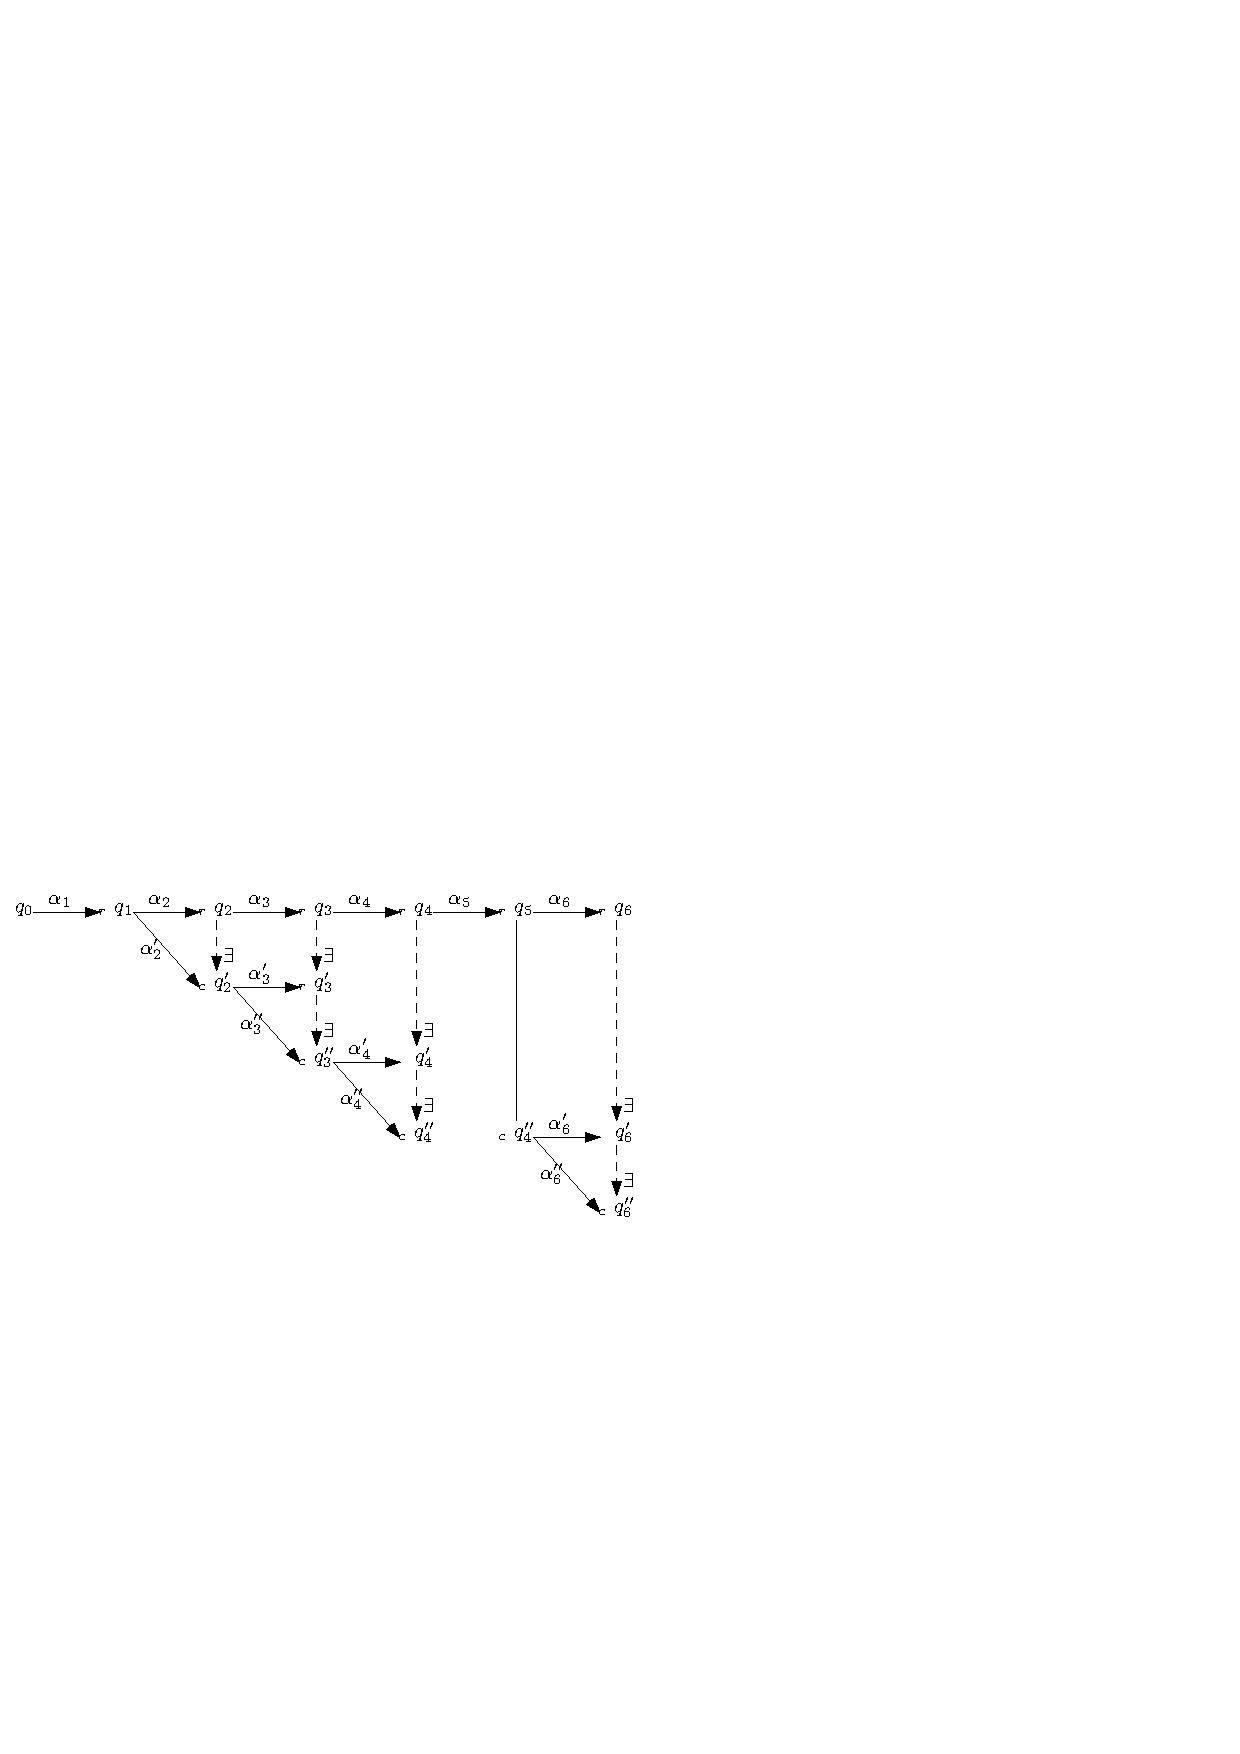
\includegraphics[width=0.6 \textwidth]{figures/PIC-Generate-AbstractTrace-NormaltoCompact.pdf}
%\vspace{-10pt}
%  \caption{The process of generate a trace of $CRImp(Spec)$ from a trace of $RImp(Spec)$}
%  \label{fig:the process of generate a trace of CRImpSpec from a trace of RImpSpec}
%\end{figure}




%{\noindent \bf Lemma \ref{lemma:RIMPSpec and CRIMPSpec have same abstract traces}}: $absT(RImp(Spec)) = absT(CRImp(Spec))$
%\begin {proof}
%The $\supseteq$ direction is obvious from the definition of $absT(CRImp(Spec))$.
%To prove the $\subseteq$ direction. Given a execution $t_1 = \alpha_1 \cdot \ldots \in \llbracket RImp(Spec) \rrbracket$. Let us show how to construct a path of $CRImp(Spec)$.
%\begin{itemize}
%\setlength{\itemsep}{0.5pt}
%\item[-] $q_1 {\xrightarrow{\alpha_2}}_r q_2$: By definition of $\rightarrow_c$, $\exists \alpha'_2$, such that $q_1 {\xrightarrow{\alpha'_2}}_c q'_2 \wedge conc(q_2)=q'_2$. Then, it is obvious that $(q_2,q'_2) \in R_{O_2}$ for some $O_2$.

%\item[-] $q_2 {\xrightarrow{\alpha_3}}_r q_3$: Since $(q_2,q'_2) \in R_{O_2} \wedge q_2 {\xrightarrow{\alpha_3}}_r q_3 $, we can see that $\exists \alpha'_3,q'_3$, such that $q'_2 {\xrightarrow{\alpha'_3}}_r q'_3 \wedge (q_3,q'_3) \in R_{O_2}$.

    %By definition of $\rightarrow_c$, $\exists \alpha''_3$, such that $q'_2 {\xrightarrow{\alpha''_3}}_c q''_3 \wedge conc(q'_3)=q''_3$. Then, it is obvious that $(q'_3,q''_3) \in R_{O_3}$ for some $O_3$. Therefore, $(q_3,q''_3) \in R_{(O_2 \cup O_3)}$.

%\item[-] If $i \geq 3 \wedge q_i {\xrightarrow{addDel(o,r)}}_r q_{i+1} \wedge o \in S_p(q_i) \cup S_m(q_i)$: We already know that $(q_i,q''_i) \in R_{O}$ for some $O$, then it is obvious that $(q_{i+1},q''_{i+1}) \in R_{O}$, where $q''_{i+1} = q''_i$.

%\item[-] If $i \geq 3 \wedge q_i {\xrightarrow{\alpha_{i+1}}}_r q_{i+1} \neg (\alpha_i = addDel(o,r) \wedge o \in S_p(q_i) \cup S_m(q_i))$: We already know that $(q_i,q''_i) \in R_{O}$ for some $O$. Since $q_i {\xrightarrow{\alpha_{i+1}}}_r q_{i+1}$, we can see that $\exists \alpha'_{i+1},q'_{i+1}$, such that $q''_i {\xrightarrow{\alpha'_{i+1}}}_r q'_{i+1} \wedge (q_{i+1},q'_{i+1}) \in R_{O}$.

    %By definition of $\rightarrow_c$, $\exists \alpha''_{i+1}$, such that $q''_i {\xrightarrow{\alpha''_{i+1}}}_c q''_{i+1} \wedge conc(q'_{i+1})=q''_{i+1}$. Then, it is obvious that $(q'_{i+1},q''_{i+1}) \in R_{O_{i+1}}$ for some $O_{i+1}$. Therefore, $(q_{i+1},q''_{i+1}) \in R_{(O \cup O_{i+1})}$.
%\end{itemize}

%\figurename~\ref{fig:the process of generate a trace of CRImpSpec from a trace of RImpSpec} given an example when (1) $q_0 {\xrightarrow{\alpha_1}}_r q_1 {\xrightarrow{\alpha_2}}_r q_2 {\xrightarrow{\alpha_3}}_r q_3 {\xrightarrow{\alpha_4}}_r q_4 {\xrightarrow{\alpha_5}}_r q_6 {\xrightarrow{\alpha_6}}_r q_6$ is a path of $RImp(Spec)$, (2) $\alpha_5=addDel(o,r) \wedge o \in S_p(q_4) \cup S_m(q_4)$, and $\forall i \neq 5$, $\neg ( \alpha_i=addDel(o,r) \wedge o \in S_p(q_{i-1}) \cup S_m(q_{i-1})$.

%It is easy to see that the abstract trace of $\alpha_1 \cdot \alpha_2 \cdot \alpha_3 \cdot \alpha_4$ in $RImp(Spec)$ is the abstract trace of $\alpha_1 \cdot \alpha'_2 \cdot \alpha''_3 \cdot \alpha''_4$ in $CRImp(Spec)$. This completes the proof of this lemma. $\qed$
%\end {proof}















\section{Definitions and Proofs of Section \ref{sec:implementation}}
\label{sec:appendix definitions and proofs of section implementation}



{\noindent \bf Lemma \ref{lemma:semantics of imp cd contains the set of causal delivery executions of semantics of imp}}: $\llbracket imp \rrbracket_{cd} = \{ t \vert t \in \llbracket imp \rrbracket \wedge t$ satisfies causal delivery $\}$.

\begin {proof}

Given $t = \alpha_1 \cdot \ldots \in \llbracket imp \rrbracket_{cd}$, if there exists $q_1,\ldots \in Q$, such that $q_0 {\xrightarrow{\alpha_1}} q_1 {\xrightarrow{\alpha_2}} \ldots$. We need to prove the following property: On each state $q_i=(repD_i,msgs_i,<_i)$,

\begin{itemize}
\setlength{\itemsep}{0.5pt}
\item[-] $P_1$: $msgs_i = \{ (dat,r,r') \vert$ the operation generating this message is launched by replica $r$ and its message has not been applied to replica $r'$ in $t[1,i]\}$.

\item[-] $P_2$: $m_1 <_i m_2$, iff $m_1$ and $m_2$ have same destination replica, and the operation generating $m_1$ happens before the operation generating $m_2$ in $t[1,i]$.

\item[-] $P_3$: $m <_i r$, iff the destination replica of $m$ is not $r$, and the operation generating $m$ is visible to replica $r$ in $t[1,i]$, and does not happen before ``any operation that launched by replica $r$'' in $t[1,i]$.
\end{itemize}

Once we prove that $P_1$, $P_2$ and $P_3$ holds for each $q_i$, let us prove this lemma by contradiction: Assume that update operations $o_1 <_{hb} o_2$, messages of $o_1$ are $\{ (d_1,r_1,\_) \}$, messages of $o_2$ are \{ $(d_2,r_2,\_) \}$, $\alpha_i = apply((d_2,r_2,r'),r')$, $\alpha_j = apply((d_1,r_1,r'),r')$, and $i<j$. Then in $q_i=(repD_i,msgs_i,<_i)$, since $o_1 <_{hb} o_2$ and transition rules of $\llbracket imp \rrbracket_{cd}$, we could not launch $apply((d_2,r_2,r'),r')$ transition, which is the contradiction.



Let us begin to prove that each state $q_i=(repD_i,msgs_i,<_i)$ satisfies properties $P_1$, $P_2$ and $P_3$. We prove this by induction on $t$.

\begin{itemize}
\setlength{\itemsep}{0.5pt}
\item[-] It is obvious that $q_0$ satisfies properties $P_1$, $P_2$ and $P_3$.

\item[-] Since $\alpha_1$ must be either a query transition or an update transition, it is easy to see that $<_1 = \emptyset$ and $q_1$ satisfies properties $P_1$, $P_2$ and $P_3$.

\item[-] Assume that $q_i=(repD_i,msgs_i,<_i)$ satisfies properties $P_1$, $P_2$ and $P_3$. let us consider $q_{i+1}= (repD_{i+1},msgs_{i+1},<_{i+1})$,

    \begin{itemize}
    \setlength{\itemsep}{0.5pt}
    \item[-] If $q_{i+1}$ is obtained from $q_i$ by a query transition, then this holds obviously.

    \item[-] Else, if $q_{i+1}$ is obtained from $q_i$ by a update transition. Then we can see that $(repD_i,msgs_i,<_i) {\xrightarrow{m(a,b,r)}} (repD_{i+1},msgs_{i+1}=msgs \cup \{ (dat,r,r') \vert  r' \in RId \wedge r \neq r' \},<_{i+1} = <_i \otimes dat)$.

        Since we add messages $\{ (dat,r,r') \vert  r' \in RId \wedge r \neq r' \}$ into $msgs_i$, we can see that $P_1$ holds.

        To satisfy $P_2$ and $P_3$, we need to make newly add messages maximal w.r.t $<$ and still keep transitivity, which is done by $<_i \otimes dat$.

    \item[-] Else, $q_{i+1}$ is obtained from $q_i$ by a applying transition. Then we can see that $(repD_i,msgs_i,<_i) {\xrightarrow{apply(m=(dat,r_1,r))}} (repD_{i+1},msgs_{i+1} = msgs_i - \{ m \}, <_{i+1} = <_i \otimes m )$, where $m$ is minimal w.r.t $<_i$ among messages in $msgs_i(r)$.

        Since we use one message $m$ in this process and remove it from $msgs_i$, we can see that $P_1$ holds.

        Applying message will introduce new visibility relation. To satisfy $P_2$ and $P_3$, we need to first forget $m$, record the newly introduced visibility relation, and still keep transitivity. This is done by $<_i \otimes m$.
    \end{itemize}
\end{itemize}

This completes the proof of this lemma. $\qed$
\end {proof}

















\forget
{

\section{Definitions of Section \ref{sec:specifications and consistencies}}
\label{sec:appendix definitions of section specifications and consistencies}

Let us give the definition of specification $S_{\textit{list}}$ of distributed list specification. $(O,<,<_{\textit{arb}}) \in S_{\textit{list}}(x)$, if

\begin{itemize}
\setlength{\itemsep}{0.5pt}
\item[-] $<^{-1}$ contains finite elements, $<$ is acyclic and $<_{\textit{arb}}$ is a total order of $add$ operations in $O \cup \{ o \}$, where $o \notin O$ and $o$ is in domain of $<_{\textit{arb}}$. By definition of poset we can see that $cont(o)=x$. Let $KnownRemoved=\emptyset$.

\item[-] Step $1$: For each minimal operation $o_1$ w.r.t $<$, let $Op(o_1)=\{ o_1 \}$, $seq(o_1)$ be obtained by ordering elements of $Op(o_1)$ with $<_{\textit{arb}}$ order. We require $cont(o_1)=add(\_,1)$.

\item[-] Step $i+1$: For each $o_2$, which are immediate successor of some $o_1$ of step $i$.

    If $<^{-1}(o_2)$ does not contain $rem$ operations:

    \begin{itemize}
    \setlength{\itemsep}{0.5pt}
    \item[-] Let $Op(o_2)$ be the set of $add$ operations in $<^{-1}(o_2) \cup \{ o_2 \}$, and let $seq(o_2)$ be obtained by ordering elements of $Op(o_2)$ with $<_{\textit{arb}}$ order.

    \item[-] If $cont(o_2) = add(a,pos)$, then $seq(o_2)[pos] = o_2$.

    \item[-] Else, if $cont(o_2) = rem(pos,a)$, then $cont(seq(o_2)[pos])=add(a,\_)$. Let $o_a=seq(o_2)[pos]$. Let $KnownRemoved = KnownRemoved \cup \{ (o_a,o_2) \}$.
    \end{itemize}

    If $<^{-1}(o_2)$ contains $rem$ operations:

    \begin{itemize}
    \setlength{\itemsep}{0.5pt}
    \item[-] Let $O_r$ be the set of $rem$ operations in $<^{-1}(o_2)$. According to our construction, $\forall o_r \in O_r$, $\exists o_p$, such that $(o_p,o_r) \in KnownRemoved$.

    \item[-] Let $Op(o_2) = \{ o' \vert o'$ is a $add$ operation in $<^{-1}(o_2) \cup \{ o_2 \} \} - \{ o'_p \vert \exists o', (o'_p,o') \in KnownRemoved \}$. Let $seq(o_2)$ be obtained by ordering elements of $Op(o_2)$ with $<_{\textit{arb}}$ order.

    \item[-] If $cont(o_2) = add(a,pos)$, then $seq(o_2)[pos] = o_2$.

    \item[-] Else, if $cont(o_2) = rem(pos,a)$, then $cont(seq(o_2)[pos])=add(a,\_)$. Let $o_a=seq(o_2)[pos]$. Let $KnownRemoved = KnownRemoved \cup \{ (o_a,o_2) \}$.
    \end{itemize}

\item[-] Assume we have investigated all operations in $O$.

    \begin{itemize}
    \setlength{\itemsep}{0.5pt}
    \item[-] Let $O_r$ be the set of $rem$ operations in $O$. According to our construction, $\forall o_r \in O_r$, $\exists o_p$, such that $(o_p,o_r) \in KnownRemoved$.

    \item[-] Let $Op(o) = \{ o' \vert o'$ is a $add$ operation in $O \cup \{ o \} \} - \{ o'_p \vert \exists o', (o'_p,o') \in KnownRemoved \}$. Let $seq(o)$ be obtained by ordering elements of $Op(o)$ with $<_{\textit{arb}}$ order.

    \item[-] If $cont(o) = add(a,pos)$, then $seq(o)[pos] = o$.

    \item[-] Else, if $cont(o) = rem(pos,a)$, then $cont(seq(o_2)[pos])=add(a,\_)$.

    \item[-] Else, if $cont(o)=read(\top,l)$, then is the sequence of operation contents of $seq(o)$.
    \end{itemize}
\end{itemize}


\begin{itemize}
\item[-] We check correctness of operations of $O$ with a procedure: Let $O_k$ be the operations we have already checked, and $KR$ record pairs $(o_1,o_2)$ such that the item added by $o_1$ have been removed by $o_2$. At the beginning, $O_k = \emptyset$ and $KR = \emptyset$. Then in each loop,

    \begin{itemize}
    \setlength{\itemsep}{0.5pt}
    \item[-] Let $O_k = O_k \cup \{ o_1 \}$, where $<^{-1}(o_1) \subseteq O_k$.

    \item[-] Let $O_r$ be the set of $rem$ operations in $<^{-1}(o_1)$. %According to our construction, $\forall o_r \in O_r$, $\exists o_p$, such that $(o_p,o_r) \in KnownRemoved$.

    \item[-] Let $Op(o_1) = \{ o_2 \vert lab(o_2)=add(\_,\_) \in <^{-1}(o_1) \cup \{ o_1 \} \} - \{ o_3 \vert \exists o_4, (o_3,o_4) \in KR \}$. Let $seq(o_1)$ be obtained by ordering elements of $Op(o_1)$ with $arb$ order.

    \item[-] If $lab(o_1) = rem(pos,a)$, then we require that $lab(seq(o_1)[pos])=add(a,\_)$, and change $KR$ into $KR \cup \{ (seq(o_1)[pos],o_1) \}$.

    \item[-] Else, if $lab(o_1) = add(a,pos)$, then we require that $seq(o_1)[pos] = o_1$.
    \end{itemize}

    We require that this procedure be terminated with $O_k = O$.

\item[-] {\color {red}Let $Op(o) = \{ o_1 \vert lab(o_1)=add(\_,\_) \in <^{-1}(o) \cup \{ o \} \} - \{ o_2 \vert \exists o_3, (o_2,o_3) \in KR \}$, and let $seq(o)$ be obtained by ordering elements of $Op(o)$ with $arb$ order.}

    \begin{itemize}
    \setlength{\itemsep}{0.5pt}
    \item[-] If $lab(o)=add(a,pos)$, then we require that $seq(o)[pos]=o$.

    \item[-] Else, if $lab(o)=rem(pos,a)$, then we require that $lab(seq(o)[pos]) = add(a,\_)$.

    \item[-] Else, if $lab(o)=read(\top,list)$, then $list$ is the sequence of operation labels of seq(o).
    \end{itemize}
\end{itemize}


\section{Definitions and Proofs of Section \ref{sec:reference implementation}}
\label{sec:appendix definitions and proofs of section reference implementation}



\subsection{Proof of Lemma \ref{lemma:executions of reference implementation are eventual consistent}}
\label{subsec:appendix proof of lemma executions of reference implementation are eventual consistent}

{\noindent \bf Lemma \ref{lemma:executions of reference implementation are eventual consistent}}: $\forall t \in \llbracket RImp(Spec) \rrbracket$, $poSet(t)$ is eventual consistent w.r.t $Spec$.

\begin {proof}

Assume $RImp(Spec) = (Q,\Sigma,vis,,q_0,li,\rightarrow,livReq)$, let $t = \alpha_1, \ldots, $ and $\exists q_1,\ldots$, such that $q_0 {\xrightarrow{\alpha_1}} q_1 {\xrightarrow{\alpha_2}} \ldots$, and $livReq(t) = \textit{true}$. Let $poSet(t)=(O_t,<_t)$. Let $gi = (O_t,<_{gi})$ be the global interpretation of $t$.

For each operation $o$, assume $o$ is first introduced by a transition from $q_i$ to $q_{i+1}$, then, the local interpretation of $o$ is $li(q_i,r)$, where $r$ is the replica of $o$.

We prove this lemma by consider the four requirements individually:

\begin{itemize}
\setlength{\itemsep}{0.5pt}
\item[-] $\textit{GIpf}$: Let us consider two kinds of operations $o$.

If $\exists o'$, such that $o' <_{gi} o$, then $\exists i < j$, such that $o'$ and $o$ are the operations of $\alpha_i$ and $\alpha_j$, respectively, and one of the following cases holds: (1) $o'$ and $o$ are of same replica, or (2) $\exists i', i < i' < j$, $\alpha_{i'}=addDel(o',r')$ and $r'$ is the replica of $o$. In each case, it is easy to see that $<^{-1}_{gi}(o)$ contains lee or equal operations than the set of operations in $t[1,j]$ and its number is obviously finite.

    If $\neg \exists o'$, such that $o' <_{gi} o$, then it is easy to see that $o$ is the first operation of its replica and no operation is delivered to that replica before $o$. In this case, it is obvious that $<^{-1}_{gi}(o)$ is finite.

\item[-] $\textit{THINAIR}$: According to the definition, we could see that on each state $q_i$, local interpretation is a subset of visibility relation, and $ro$ is also a subset of visibility relation. It is easy to prove that on each state, $vis$ is acyclic.

\item[-] $\textit{RVAL}$: We only need to consider query operations for $\textit{RVAL}$ property, since only query operations have return values. According to construction of $\llbracket RImp(Spec) \rrbracket$, to launch a query operation $(m,a,b,rid,oid)$ transition of replica $r$ from state $q_i$, we already check whether $li(q_i,r)$, the local interpretation w.r.t $q_i$ and $r$, is in $Spec(m,a,b)$.

\item[-] $\textit{EVENTUAL}$: Let $P=(O_P,<_P)$ be a finite prefix of $gi$.

We can see that $<_P$ is the visibility relation of operations in $O_P$. Let $O'_P = \{ o \vert \exists o_1,o_2 \in O_P,$ $o_1$ is visible to $o_2$ via $o'_1,\ldots,o'_m$, and $o \in \{ o'_1,\ldots,o'_n \} \}$. It is easy to see that $O'_P$ is finite, and assume that operations of $O_P \cup O'_P$ are chosen before $\alpha_{idx}$

Since $livReq(t)=true$, $\exists idx1$, such that in $t[1,idx1]$, all operations in $t[1,idx]$ has been delivered to every replica. According to our construction of $li$, this implies that for each state after $\alpha_{idx1}$ and each replica (1) its local interpretation contains $O_P$ and $O'_P$, and (2) the relation of local interpretation then contains the visibility relation between operations in $O_P$.
\end{itemize}

This completes the proof of this lemma. $\qed$
\end {proof}








\section{Definitions and Proofs of Section \ref{sec:implementation}}
\label{sec:appendix definitions and proofs of section implementation}



{\noindent \bf Lemma \ref{lemma:semantics of imp cd contains the set of causal delivery executions of semantics of imp}}: $\llbracket imp \rrbracket_{cd} = \{ t \vert t \in \llbracket imp \rrbracket \wedge t$ satisfies causal delivery $\}$.

\begin {proof}

Given $t = \alpha_1 \cdot \ldots \in \llbracket imp \rrbracket_{cd}$, if there exists $q_1,\ldots \in Q$, such that $q_0 {\xrightarrow{\alpha_1}} q_1 {\xrightarrow{\alpha_2}} \ldots$. We need to prove the following property: On each state $q_i=(repD_i,msgs_i,<_i)$,

\begin{itemize}
\setlength{\itemsep}{0.5pt}
\item[-] $P_1$: $msgs_i = \{ (dat,r,r') \vert$ the operation generating this message is launched by replica $r$ and its message has not been applied to replica $r'$ in $t[1,i]\}$.

\item[-] $P_2$: $m_1 <_i m_2$, iff $m_1$ and $m_2$ have same destination replica, and the operation generating $m_1$ happens before the operation generating $m_2$ in $t[1,i]$.

\item[-] $P_3$: $m <_i r$, iff the destination replica of $m$ is not $r$, and the operation generating $m$ is visible to replica $r$ in $t[1,i]$, and does not happen before ``any operation that launched by replica $r$'' in $t[1,i]$.
\end{itemize}

Once we prove that $P_1$, $P_2$ and $P_3$ holds for each $q_i$, let us prove this lemma by contradiction: Assume that update operations $o_1 <_{hb} o_2$, messages of $o_1$ are $\{ (d_1,r_1,\_) \}$, messages of $o_2$ are \{ $(d_2,r_2,\_) \}$, $\alpha_i = apply((d_2,r_2,r'),r')$, $\alpha_j = apply((d_1,r_1,r'),r')$, and $i<j$. Then in $q_i=(repD_i,msgs_i,<_i)$, since $o_1 <_{hb} o_2$ and transition rules of $\llbracket imp \rrbracket_{cd}$, we could not launch $apply((d_2,r_2,r'),r')$ transition, which is the contradiction.



Let us begin to prove that each state $q_i=(repD_i,msgs_i,<_i)$ satisfies properties $P_1$, $P_2$ and $P_3$. We prove this by induction on $t$.

\begin{itemize}
\setlength{\itemsep}{0.5pt}
\item[-] It is obvious that $q_0$ satisfies properties $P_1$, $P_2$ and $P_3$.

\item[-] Since $\alpha_1$ must be either a query transition or an update transition, it is easy to see that $<_1 = \emptyset$ and $q_1$ satisfies properties $P_1$, $P_2$ and $P_3$.

\item[-] Assume that $q_i=(repD_i,msgs_i,<_i)$ satisfies properties $P_1$, $P_2$ and $P_3$. let us consider $q_{i+1}= (repD_{i+1},msgs_{i+1},<_{i+1})$,

    \begin{itemize}
    \setlength{\itemsep}{0.5pt}
    \item[-] If $q_{i+1}$ is obtained from $q_i$ by a query transition, then this holds obviously.

    \item[-] Else, if $q_{i+1}$ is obtained from $q_i$ by a update transition. Then we can see that $(repD_i,msgs_i,<_i) {\xrightarrow{m(a,b,r)}} (repD_{i+1},msgs_{i+1}=msgs \cup \{ (dat,r,r') \vert  r' \in RId \wedge r \neq r' \},<_{i+1} = <_i \otimes dat)$.

        Since we add messages $\{ (dat,r,r') \vert  r' \in RId \wedge r \neq r' \}$ into $msgs_i$, we can see that $P_1$ holds.

        To satisfy $P_2$ and $P_3$, we need to make newly add messages maximal w.r.t $<$ and still keep transitivity, which is done by $<_i \otimes dat$.

    \item[-] Else, $q_{i+1}$ is obtained from $q_i$ by a applying transition. Then we can see that $(repD_i,msgs_i,<_i) {\xrightarrow{apply(m=(dat,r_1,r))}} (repD_{i+1},msgs_{i+1} = msgs_i - \{ m \}, <_{i+1} = <_i \otimes m )$, where $m$ is minimal w.r.t $<_i$ among messages in $msgs_i(r)$.

        Since we use one message $m$ in this process and remove it from $msgs_i$, we can see that $P_1$ holds.

        Applying message will introduce new visibility relation. To satisfy $P_2$ and $P_3$, we need to first forget $m$, record the newly introduced visibility relation, and still keep transitivity. This is done by $<_i \otimes m$.
    \end{itemize}
\end{itemize}

This completes the proof of this lemma. $\qed$
\end {proof}
}





